\chapter{Generación de lenguaje natural.}
\label{cap:nlg_intro}
La generación de lenguaje natural (NLG) es un una rama de la lingüística computacional y la inteligencia artificial encargada de estudiar la construcción de sistemas computacionales capaces de producir texto en español o cualquier otra lengua humana a partir de algún tipo de representación no-lingüística de la información a comunicar. Estos sistema combinan conocimientos tanto del lenguaje en cuestión cómo del dominio de aplicación para producir automáticamente documentos, reportes, mensajes o cualquier otro tipo de textos.

Dentro de la comunidad desarrolladora e investigadora de la NLG hay un cierto consenso sobre la funcionalidad lingüística general de un sistema de NLG.
En este trabajo se optó por seguir la metodología más comúnmente aceptada, propuesta por Reiter y Dale\cite{reiterdale}.
A continuación describiremos brevemente los aspectos mas importantes de esta metodología y en capítulos posteriores desarrollaremos más en profundidad en los puntos mas relevantes para nuestro trabajo.

\section{Análisis de requerimientos}
El primer paso en la construcción de cualquier sistema de software, incluyendo los sistemas de generación de lenguaje natural, será el de realizar un análisis de requerimientos y a partir de ahí generar una especificación inicial del sistema. 

Para el análisis de requerimientos, Reiter y Dale proponen realizar un \emph{corpus} de textos de ejemplo y a partir de ellos obtener una especificación para el sistema a desarrollar. Estos ejemplos estarán compuestos por una colección de datos de entrada del sistema con sus respectivas salidas (texto en lenguaje natural). Estos deberán estar redactados por un humano experto y deberían caracterizar todas las salidas posibles que se espera que el sistema genere.

En el capítulo~\ref{cap:corpus} profundizaremos más sobre este tema, describiremos y analizaremos el \emph{corpus de descripciones} utilizado para este trabajo.

\section{Tareas de la generación de lenguaje natural}

Dentro de la comunidad desarrolladora e investigadora de la generación de lenguaje natural, hay cierto consenso sobre las tareas que deben llevarse a cabo para, a partir de los datos de entrada, generar texto final en lenguaje natural. 

La más comúnmente aceptada es la clasificación de Reiter y Dale que distingue las siguientes siete tareas que deben ser realizadas a lo largo de todo el proceso: 

\bigskip
\noindent
\textbf{Determinación del contenido:} es el proceso de determinar que información debe ser comunicada en el texto final; será el encargado de que el mismo contenga toda la información requerida por el usuario. Generalmente involucra una o más tareas de selección, resumen y razonamiento con los datos de entrada.

\bigskip
\noindent
\textbf{Estructuración del documento:} es el proceso de imponer un orden y estructura sobre los textos generados a fin de que la información del documento final se encuentre estructurada de forma entendible y fácil de leer.

\bigskip
\noindent
\textbf{Lexicalización:} es el proceso de decidir que palabras y frases especificas usar para expresar los distintos conceptos y relaciones del dominio. En esta etapa se deberá establecer como se expresa un significado conceptual concreto, descrito en términos del modelo del dominio, usando elementos léxicos (sustantivos, verbos, adjetivos, etc).

\bigskip
\noindent
\textbf{Generación de expresiones de referencia:} es la tarea de elegir que expresiones usar para identificar entidades del dominio de aplicación. Podríamos querer referirnos a una determinada entidad de distintas formas. Por ejemplo: podríamos querer referirnos al mes en curso como, ``febrero'', ``este mes'', ``este'', etc.

\bigskip
\noindent
\textbf{Agregación:} se encarga de combinar dos o mas elementos informativos con el fin de conseguir un texto más fluido y legible. La agregación decide que elementos se pueden agrupar para generar oraciones mas complejas sin modificar el significado de las mismas. Por Ejemplo, dos frases de una descripción para una clase de prueba de un scheduler se podrían expresar como:
\emph{``El proceso a borrar se encuentra en la tabla de procesos. El estado del proceso a borrar es waiting.''} o \emph{``El proceso a borrar se encuentra en la tabla de procesos y el estado del mismo es waiting.''}

\bigskip
\noindent
\textbf{Realización lingüística:} es el proceso de aplicar reglas gramaticales (a estructuras generadas por las etapas anteriores) con el fin de producir un texto que sea sintáctica, morfológica y ortográficamente correcto.

\bigskip
\noindent
\textbf{Realización de la estructura:} esta tarea se encarga de convertir estructuras abstractas como párrafos y secciones (generadas por etapas anteriores) en texto comprensible por el componente de presentación del documento. Por ejemplo, la salida del sistema de NLG podría ser código LaTeX para luego ser post-procesado, en este caso sería esta etapa la encargada de agregar delimitadores y comandos de LaTeX para generar el documento. 

\section{Arquitectura para la NLG.}
Existen muchas maneras de construir un sistema que realice las tareas antes mencionadas. Una forma podría ser construir un único módulo encargado de llevar a cabo todas las tareas en simultaneo. En el otro extremo, podríamos tener un módulo separado para cada tarea y conectarlos mediante un \emph{pipeline}. En este caso, el sistema primero se encargaría de la determinación de contenido, luego la estructuración del documento, y así sucesivamente. La desventaja de este último modelo es que asume que las tareas deben ser realizadas en un único orden y que las funcionalidades de las mismas no se solapan.

En este trabajo utilizaremos la arquitectura mas comúnmente utilizada para sistemas de NLG. Esta consiste de tres módulos conectados mediante un \emph{pipeline}. La misma se encuentra en el medio de los dos extremos antes mencionados.

\begin{figure}[h]
  	\centering
	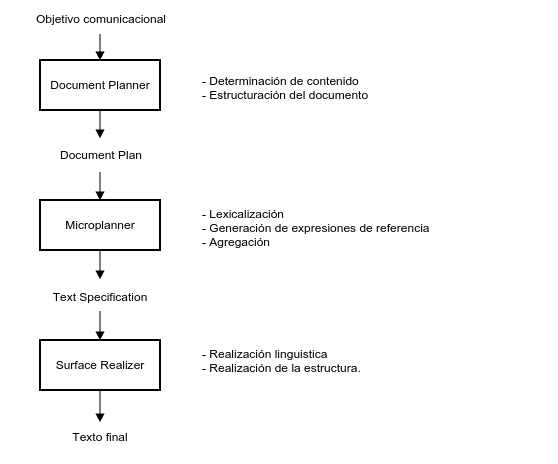
\includegraphics{img/arquitectura.png}
	\caption{Arquitectura típica sistema NLG.}
  	\label{fig:png_arquitectura}
\end{figure}

El primer módulo de nuestro sistema será el \emph{document planner}, encargado de realizar las tareas de determinación de contenido y estructuración del documento. Veremos en el capítulo~\ref{cap:document_planning} que estas tareas se encuentran sumamente relacionadas y son realizadas en simultaneo. La salida de esta etapa y entrada del \emph{microplanner} será un \emph{document plan}, este será una abstracción del documento final que contendrá los elementos informativos que se desea comunicar.

El segundo módulo será el encargado de realizar las tareas de lexicalización, generación de expresiones de referencia y agregación. La función del mismo será la de trabajar el document plan generando una especificación mas refinada del texto final, una \emph{text specification}. El \emph{microplanner} será el responsable de transformar los elementos informativos incluidos en el document plan en una especificación mas concreta de una oración. En el capítulo~\ref{cap:microplanning} desarrollaremos mas en profundidad el funcionamiento del microplanner.

Finalmente el \emph{surface realiser} tomará como entrada el text specification generado por la etapa anterior y será el encargado de producir el texto final. Este módulo deberá llevar a cabo las tareas de realización lingüística y de superficie ates mencionadas.